% Options for packages loaded elsewhere
\PassOptionsToPackage{unicode}{hyperref}
\PassOptionsToPackage{hyphens}{url}
\PassOptionsToPackage{dvipsnames,svgnames,x11names}{xcolor}
%
\documentclass[
  letterpaper,
  DIV=11,
  numbers=noendperiod]{scrartcl}

\usepackage{amsmath,amssymb}
\usepackage{lmodern}
\usepackage{iftex}
\ifPDFTeX
  \usepackage[T1]{fontenc}
  \usepackage[utf8]{inputenc}
  \usepackage{textcomp} % provide euro and other symbols
\else % if luatex or xetex
  \usepackage{unicode-math}
  \defaultfontfeatures{Scale=MatchLowercase}
  \defaultfontfeatures[\rmfamily]{Ligatures=TeX,Scale=1}
\fi
% Use upquote if available, for straight quotes in verbatim environments
\IfFileExists{upquote.sty}{\usepackage{upquote}}{}
\IfFileExists{microtype.sty}{% use microtype if available
  \usepackage[]{microtype}
  \UseMicrotypeSet[protrusion]{basicmath} % disable protrusion for tt fonts
}{}
\makeatletter
\@ifundefined{KOMAClassName}{% if non-KOMA class
  \IfFileExists{parskip.sty}{%
    \usepackage{parskip}
  }{% else
    \setlength{\parindent}{0pt}
    \setlength{\parskip}{6pt plus 2pt minus 1pt}}
}{% if KOMA class
  \KOMAoptions{parskip=half}}
\makeatother
\usepackage{xcolor}
\setlength{\emergencystretch}{3em} % prevent overfull lines
\setcounter{secnumdepth}{-\maxdimen} % remove section numbering
% Make \paragraph and \subparagraph free-standing
\ifx\paragraph\undefined\else
  \let\oldparagraph\paragraph
  \renewcommand{\paragraph}[1]{\oldparagraph{#1}\mbox{}}
\fi
\ifx\subparagraph\undefined\else
  \let\oldsubparagraph\subparagraph
  \renewcommand{\subparagraph}[1]{\oldsubparagraph{#1}\mbox{}}
\fi

\usepackage{color}
\usepackage{fancyvrb}
\newcommand{\VerbBar}{|}
\newcommand{\VERB}{\Verb[commandchars=\\\{\}]}
\DefineVerbatimEnvironment{Highlighting}{Verbatim}{commandchars=\\\{\}}
% Add ',fontsize=\small' for more characters per line
\usepackage{framed}
\definecolor{shadecolor}{RGB}{241,243,245}
\newenvironment{Shaded}{\begin{snugshade}}{\end{snugshade}}
\newcommand{\AlertTok}[1]{\textcolor[rgb]{0.68,0.00,0.00}{#1}}
\newcommand{\AnnotationTok}[1]{\textcolor[rgb]{0.37,0.37,0.37}{#1}}
\newcommand{\AttributeTok}[1]{\textcolor[rgb]{0.40,0.45,0.13}{#1}}
\newcommand{\BaseNTok}[1]{\textcolor[rgb]{0.68,0.00,0.00}{#1}}
\newcommand{\BuiltInTok}[1]{\textcolor[rgb]{0.00,0.23,0.31}{#1}}
\newcommand{\CharTok}[1]{\textcolor[rgb]{0.13,0.47,0.30}{#1}}
\newcommand{\CommentTok}[1]{\textcolor[rgb]{0.37,0.37,0.37}{#1}}
\newcommand{\CommentVarTok}[1]{\textcolor[rgb]{0.37,0.37,0.37}{\textit{#1}}}
\newcommand{\ConstantTok}[1]{\textcolor[rgb]{0.56,0.35,0.01}{#1}}
\newcommand{\ControlFlowTok}[1]{\textcolor[rgb]{0.00,0.23,0.31}{#1}}
\newcommand{\DataTypeTok}[1]{\textcolor[rgb]{0.68,0.00,0.00}{#1}}
\newcommand{\DecValTok}[1]{\textcolor[rgb]{0.68,0.00,0.00}{#1}}
\newcommand{\DocumentationTok}[1]{\textcolor[rgb]{0.37,0.37,0.37}{\textit{#1}}}
\newcommand{\ErrorTok}[1]{\textcolor[rgb]{0.68,0.00,0.00}{#1}}
\newcommand{\ExtensionTok}[1]{\textcolor[rgb]{0.00,0.23,0.31}{#1}}
\newcommand{\FloatTok}[1]{\textcolor[rgb]{0.68,0.00,0.00}{#1}}
\newcommand{\FunctionTok}[1]{\textcolor[rgb]{0.28,0.35,0.67}{#1}}
\newcommand{\ImportTok}[1]{\textcolor[rgb]{0.00,0.46,0.62}{#1}}
\newcommand{\InformationTok}[1]{\textcolor[rgb]{0.37,0.37,0.37}{#1}}
\newcommand{\KeywordTok}[1]{\textcolor[rgb]{0.00,0.23,0.31}{#1}}
\newcommand{\NormalTok}[1]{\textcolor[rgb]{0.00,0.23,0.31}{#1}}
\newcommand{\OperatorTok}[1]{\textcolor[rgb]{0.37,0.37,0.37}{#1}}
\newcommand{\OtherTok}[1]{\textcolor[rgb]{0.00,0.23,0.31}{#1}}
\newcommand{\PreprocessorTok}[1]{\textcolor[rgb]{0.68,0.00,0.00}{#1}}
\newcommand{\RegionMarkerTok}[1]{\textcolor[rgb]{0.00,0.23,0.31}{#1}}
\newcommand{\SpecialCharTok}[1]{\textcolor[rgb]{0.37,0.37,0.37}{#1}}
\newcommand{\SpecialStringTok}[1]{\textcolor[rgb]{0.13,0.47,0.30}{#1}}
\newcommand{\StringTok}[1]{\textcolor[rgb]{0.13,0.47,0.30}{#1}}
\newcommand{\VariableTok}[1]{\textcolor[rgb]{0.07,0.07,0.07}{#1}}
\newcommand{\VerbatimStringTok}[1]{\textcolor[rgb]{0.13,0.47,0.30}{#1}}
\newcommand{\WarningTok}[1]{\textcolor[rgb]{0.37,0.37,0.37}{\textit{#1}}}

\providecommand{\tightlist}{%
  \setlength{\itemsep}{0pt}\setlength{\parskip}{0pt}}\usepackage{longtable,booktabs,array}
\usepackage{calc} % for calculating minipage widths
% Correct order of tables after \paragraph or \subparagraph
\usepackage{etoolbox}
\makeatletter
\patchcmd\longtable{\par}{\if@noskipsec\mbox{}\fi\par}{}{}
\makeatother
% Allow footnotes in longtable head/foot
\IfFileExists{footnotehyper.sty}{\usepackage{footnotehyper}}{\usepackage{footnote}}
\makesavenoteenv{longtable}
\usepackage{graphicx}
\makeatletter
\def\maxwidth{\ifdim\Gin@nat@width>\linewidth\linewidth\else\Gin@nat@width\fi}
\def\maxheight{\ifdim\Gin@nat@height>\textheight\textheight\else\Gin@nat@height\fi}
\makeatother
% Scale images if necessary, so that they will not overflow the page
% margins by default, and it is still possible to overwrite the defaults
% using explicit options in \includegraphics[width, height, ...]{}
\setkeys{Gin}{width=\maxwidth,height=\maxheight,keepaspectratio}
% Set default figure placement to htbp
\makeatletter
\def\fps@figure{htbp}
\makeatother
\newlength{\cslhangindent}
\setlength{\cslhangindent}{1.5em}
\newlength{\csllabelwidth}
\setlength{\csllabelwidth}{3em}
\newlength{\cslentryspacingunit} % times entry-spacing
\setlength{\cslentryspacingunit}{\parskip}
\newenvironment{CSLReferences}[2] % #1 hanging-ident, #2 entry spacing
 {% don't indent paragraphs
  \setlength{\parindent}{0pt}
  % turn on hanging indent if param 1 is 1
  \ifodd #1
  \let\oldpar\par
  \def\par{\hangindent=\cslhangindent\oldpar}
  \fi
  % set entry spacing
  \setlength{\parskip}{#2\cslentryspacingunit}
 }%
 {}
\usepackage{calc}
\newcommand{\CSLBlock}[1]{#1\hfill\break}
\newcommand{\CSLLeftMargin}[1]{\parbox[t]{\csllabelwidth}{#1}}
\newcommand{\CSLRightInline}[1]{\parbox[t]{\linewidth - \csllabelwidth}{#1}\break}
\newcommand{\CSLIndent}[1]{\hspace{\cslhangindent}#1}

\KOMAoption{captions}{tableheading}
\makeatletter
\makeatother
\makeatletter
\makeatother
\makeatletter
\@ifpackageloaded{caption}{}{\usepackage{caption}}
\AtBeginDocument{%
\ifdefined\contentsname
  \renewcommand*\contentsname{Table of contents}
\else
  \newcommand\contentsname{Table of contents}
\fi
\ifdefined\listfigurename
  \renewcommand*\listfigurename{List of Figures}
\else
  \newcommand\listfigurename{List of Figures}
\fi
\ifdefined\listtablename
  \renewcommand*\listtablename{List of Tables}
\else
  \newcommand\listtablename{List of Tables}
\fi
\ifdefined\figurename
  \renewcommand*\figurename{Figure}
\else
  \newcommand\figurename{Figure}
\fi
\ifdefined\tablename
  \renewcommand*\tablename{Table}
\else
  \newcommand\tablename{Table}
\fi
}
\@ifpackageloaded{float}{}{\usepackage{float}}
\floatstyle{ruled}
\@ifundefined{c@chapter}{\newfloat{codelisting}{h}{lop}}{\newfloat{codelisting}{h}{lop}[chapter]}
\floatname{codelisting}{Listing}
\newcommand*\listoflistings{\listof{codelisting}{List of Listings}}
\makeatother
\makeatletter
\@ifpackageloaded{caption}{}{\usepackage{caption}}
\@ifpackageloaded{subcaption}{}{\usepackage{subcaption}}
\makeatother
\makeatletter
\@ifpackageloaded{tcolorbox}{}{\usepackage[many]{tcolorbox}}
\makeatother
\makeatletter
\@ifundefined{shadecolor}{\definecolor{shadecolor}{rgb}{.97, .97, .97}}
\makeatother
\makeatletter
\makeatother
\ifLuaTeX
  \usepackage{selnolig}  % disable illegal ligatures
\fi
\IfFileExists{bookmark.sty}{\usepackage{bookmark}}{\usepackage{hyperref}}
\IfFileExists{xurl.sty}{\usepackage{xurl}}{} % add URL line breaks if available
\urlstyle{same} % disable monospaced font for URLs
\hypersetup{
  pdftitle={Assignment: Game of Thrones Season Summary},
  pdfauthor={Adam Foster},
  colorlinks=true,
  linkcolor={blue},
  filecolor={Maroon},
  citecolor={Blue},
  urlcolor={Blue},
  pdfcreator={LaTeX via pandoc}}

\title{Assignment: Game of Thrones Season Summary}
\author{Adam Foster}
\date{3/5/23}

\begin{document}
\maketitle
\ifdefined\Shaded\renewenvironment{Shaded}{\begin{tcolorbox}[enhanced, borderline west={3pt}{0pt}{shadecolor}, frame hidden, boxrule=0pt, sharp corners, breakable, interior hidden]}{\end{tcolorbox}}\fi

\begin{Shaded}
\begin{Highlighting}[]
\NormalTok{season\_i }\OtherTok{=} \FunctionTok{paste}\NormalTok{(}\StringTok{"../Data/"}\NormalTok{, params}\SpecialCharTok{$}\NormalTok{season, }\StringTok{".RData"}\NormalTok{, }\AttributeTok{sep =} \StringTok{""}\NormalTok{)}
\FunctionTok{load}\NormalTok{(season\_i)}
\end{Highlighting}
\end{Shaded}

\hypertarget{game-of-thrones---season-summary-in-numbers}{%
\section{Game of Thrones - Season summary in
numbers}\label{game-of-thrones---season-summary-in-numbers}}

\hypertarget{warning-spoilers-ahead}{%
\subsubsection{\texorpdfstring{\textbf{(\emph{Warning:} spoilers
ahead)}}{(Warning: spoilers ahead)}}\label{warning-spoilers-ahead}}

\begin{center}\rule{0.5\linewidth}{0.5pt}\end{center}

\hypertarget{overview}{%
\subsubsection{Overview}\label{overview}}

(Wikipedia 2023) Game of Thrones is an American fantasy drama television
series created by David Benioff and D. B. Weiss for HBO. It is an
adaptation of A Song of Ice and Fire, a series of fantasy novels by
George R. R. Martin, the first of which is A Game of Thrones.

Set on the fictional continents of Westeros and Essos, Game of Thrones
has a large ensemble cast and follows several story arcs throughout the
course of the show. A major arc concerns the Iron Throne of the Seven
Kingdoms of Westeros through a web of political conflicts among the
noble families either vying to claim the throne or fighting for
independence from it. Another focuses on the last descendant of the
realm's deposed ruling dynasty, who has been exiled to Essos and is
plotting a return to the throne. A third story arc follows the Night's
Watch, a military order defending the realm against threats from the
North.

\begin{center}\rule{0.5\linewidth}{0.5pt}\end{center}

\hypertarget{season-summary}{%
\subsubsection{Season summary}\label{season-summary}}

\begin{Shaded}
\begin{Highlighting}[]
\CommentTok{\# setwd("..")}
\CommentTok{\# season = "season\_1"}
\CommentTok{\# path\_name = paste(getwd(), "/Data/", season, ".csv", sep = "")}
\CommentTok{\# data = read.csv(path\_name)}

\NormalTok{number\_episodes }\OtherTok{=} \FunctionTok{nrow}\NormalTok{(season\_data)}

\NormalTok{dates }\OtherTok{=} \FunctionTok{as.list}\NormalTok{(season\_data[}\StringTok{"premiere\_date"}\NormalTok{])}
\FunctionTok{library}\NormalTok{(stringr)}
\NormalTok{season\_start }\OtherTok{=} \FunctionTok{format}\NormalTok{(}\FunctionTok{as.Date}\NormalTok{(}\FunctionTok{str\_sub}\NormalTok{(dates[[}\DecValTok{1}\NormalTok{]][}\DecValTok{1}\NormalTok{], }\SpecialCharTok{{-}}\DecValTok{12}\NormalTok{, }\SpecialCharTok{{-}}\DecValTok{1}\NormalTok{), }\StringTok{"(\%Y{-}\%m{-}\%d"}\NormalTok{), }\StringTok{"\%d \%B \%Y"}\NormalTok{)}
\NormalTok{season\_end }\OtherTok{=} \FunctionTok{format}\NormalTok{(}\FunctionTok{as.Date}\NormalTok{(}\FunctionTok{str\_sub}\NormalTok{(dates[[}\DecValTok{1}\NormalTok{]][number\_episodes], }\SpecialCharTok{{-}}\DecValTok{12}\NormalTok{, }\SpecialCharTok{{-}}\DecValTok{1}\NormalTok{), }\StringTok{"(\%Y{-}\%m{-}\%d"}\NormalTok{), }\StringTok{"\%d \%B \%Y"}\NormalTok{)}

\NormalTok{viewers\_mean }\OtherTok{=} \FunctionTok{mean}\NormalTok{(}\FunctionTok{as.list}\NormalTok{(season\_data[}\StringTok{"viewers"}\NormalTok{])[[}\DecValTok{1}\NormalTok{]])}
\NormalTok{viewers\_start }\OtherTok{=} \FunctionTok{as.list}\NormalTok{(season\_data[}\StringTok{"viewers"}\NormalTok{])[[}\DecValTok{1}\NormalTok{]][}\DecValTok{1}\NormalTok{]}
\NormalTok{viewers\_end }\OtherTok{=} \FunctionTok{as.list}\NormalTok{(season\_data[}\StringTok{"viewers"}\NormalTok{])[[}\DecValTok{1}\NormalTok{]][number\_episodes]}

\NormalTok{viewers\_max }\OtherTok{=} \FunctionTok{max}\NormalTok{(}\FunctionTok{as.list}\NormalTok{(season\_data[}\StringTok{"viewers"}\NormalTok{])[[}\DecValTok{1}\NormalTok{]])}
\NormalTok{data\_popular }\OtherTok{=} \FunctionTok{subset}\NormalTok{(season\_data, viewers }\SpecialCharTok{==}\NormalTok{ viewers\_max, }\AttributeTok{select =} \FunctionTok{c}\NormalTok{(}\StringTok{"title"}\NormalTok{, }\StringTok{"description"}\NormalTok{))}
\NormalTok{data\_popular\_title }\OtherTok{=}\NormalTok{ data\_popular[[}\DecValTok{1}\NormalTok{]]}
\NormalTok{data\_popular\_description }\OtherTok{=}\NormalTok{ data\_popular[[}\DecValTok{2}\NormalTok{]]}
\end{Highlighting}
\end{Shaded}

The season of Game of Thrones consisted of 6 episodes that aired between
14 April 2019 and 19 May 2019 on HBO. The show gathered an average of
11.95 million first-day TV viewers in the US, with the number changing
from 11.7 to 13.6 million by the end of the season.

The most popular episode of the season was ``The Iron Throne'', in
which:

\begin{quote}
Jon is appalled when the Unsullied execute captured soldiers upon
Daenerys' orders. Tyrion finds Jaime and Cersei dead in the ruins.
Daenerys rallies the Unsullied and Dothraki, proclaiming she will lead
them to ``liberate'' the entire world. Tyrion resigns as Hand of the
Queen and is imprisoned for treason. Arya and Tyrion separately warn Jon
that Daenerys is a threat to him, House Stark, and the people. Jon
confronts Daenerys. Unable to halt her destructive path, an agonized Jon
kills her. Drogon, enraged, melts the Iron Throne, then carries away
Daenerys' body. Later, Tyrion proposes that all future monarchs be
chosen by Westerosi leaders, rather than familial succession. Bran Stark
is proclaimed King Bran the Broken. He grants the North independence as
a kingdom and appoints Tyrion his Hand. Jon is sentenced to the Night's
Watch to appease the Unsullied, who set sail for Naath, Missandei's
homeland. Tyrion reorganizes the Small Council -- Brienne, Bronn, Davos,
and Sam -- to rebuild King's Landing. Podrick is knighted. Sansa is
crowned Queen in the North. Arya sets sail to explore unknown lands west
of Westeros. Jon rejoins Tormund and Ghost at Castle Black, leading the
Wildlings north of the Wall.
\end{quote}

\begin{center}\rule{0.5\linewidth}{0.5pt}\end{center}

You can see how the viewership of the episodes changed in Figure 1.

\begin{Shaded}
\begin{Highlighting}[]
\FunctionTok{plot}\NormalTok{(season\_data}\SpecialCharTok{$}\NormalTok{viewers, }\AttributeTok{type=}\StringTok{"l"}\NormalTok{, }\AttributeTok{col=}\StringTok{"red"}\NormalTok{, }\AttributeTok{lwd=}\DecValTok{5}\NormalTok{, }\AttributeTok{xlab =} \StringTok{"Episode number"}\NormalTok{, }\AttributeTok{ylab =} \StringTok{"1st day TV viewers in the US (millions)"}\NormalTok{)}
\end{Highlighting}
\end{Shaded}

\begin{figure}[H]

{\centering 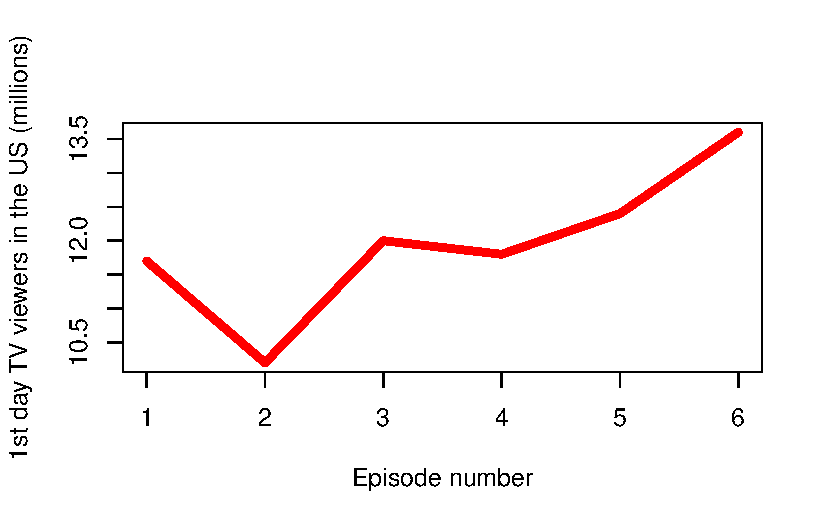
\includegraphics{Assignment_files/figure-pdf/viewers_plot-1.pdf}

}

\end{figure}

\begin{center}\rule{0.5\linewidth}{0.5pt}\end{center}

Finally, the episodes with the above-average viewership were:

\begin{Shaded}
\begin{Highlighting}[]
\NormalTok{data\_above\_mean }\OtherTok{=} \FunctionTok{subset}\NormalTok{(season\_data, viewers }\SpecialCharTok{\textgreater{}}\NormalTok{ viewers\_mean, }\AttributeTok{select =} \FunctionTok{c}\NormalTok{(}\StringTok{"no\_season"}\NormalTok{, }\StringTok{"title"}\NormalTok{, }\StringTok{"directed\_by"}\NormalTok{))}
\FunctionTok{print}\NormalTok{(data\_above\_mean)}
\end{Highlighting}
\end{Shaded}

\begin{verbatim}
   no_season             title                 directed_by
5          3  "The Long Night"            Miguel Sapochnik
9          5       "The Bells"            Miguel Sapochnik
11         6 "The Iron Throne" David Benioff & D. B. Weiss
\end{verbatim}

\hypertarget{refs}{}
\begin{CSLReferences}{1}{0}
\leavevmode\vadjust pre{\hypertarget{ref-got}{}}%
Wikipedia. 2023. {``Game of Thrones.''}
\url{https://en.wikipedia.org/wiki/Game_of_Thrones\#Premise}.

\end{CSLReferences}



\end{document}
